\documentclass[runningheads]{llncs}

\usepackage[T1]{fontenc}
\usepackage{lmodern}
\usepackage{graphicx}
\usepackage{booktabs}
\usepackage{multirow}
\usepackage{array}
\usepackage{amsmath}
\usepackage{amssymb}
\usepackage{xcolor}
\usepackage{listings}
\usepackage{tikz}
\usetikzlibrary{arrows.meta,positioning,shapes.geometric,calc,fit,backgrounds}
\usepackage{hyperref}
\hypersetup{hidelinks}
\usepackage{microtype}

% Tighten the (already \small) LNCS bibliography's inter-item spacing just enough to
% keep all references within the page budget (visual style otherwise unchanged).
\let\oldthebibliography\thebibliography
\renewcommand{\thebibliography}[1]{%
  \oldthebibliography{#1}%
  \setlength{\itemsep}{0pt plus 0.3pt}%
  \setlength{\parsep}{0pt}%
}

\raggedbottom   % collect slack at the page bottom, not between paragraphs

% let floats settle near their reference instead of drifting to the end
\renewcommand{\topfraction}{0.9}
\renewcommand{\bottomfraction}{0.8}
\renewcommand{\textfraction}{0.07}
\renewcommand{\floatpagefraction}{0.75}
\setcounter{topnumber}{3}
\setcounter{totalnumber}{5}

% last-resort glue so long monospace identifiers never push into the margin
\setlength{\emergencystretch}{3em}

% ---- colours -----------------------------------------------------------
\definecolor{kw}{RGB}{0,86,179}
\definecolor{str}{RGB}{163,21,21}
\definecolor{cmt}{RGB}{0,128,0}
\definecolor{bg}{RGB}{248,248,248}
\definecolor{rule}{RGB}{120,120,120}

% ---- diagnostic code macro --------------------------------------------
\newcommand{\code}[1]{\textsf{\small #1}}
\newcommand{\tool}{\textsc{StepCheck}}
\newcommand{\asl}{\textsc{Asl}}

% ---- listings ----------------------------------------------------------
\lstdefinestyle{base}{
  basicstyle=\ttfamily\footnotesize,
  backgroundcolor=\color{bg},
  frame=single, framesep=4pt, rulecolor=\color{rule!40},
  breaklines=true, columns=fullflexible, keepspaces=true,
  showstringspaces=false, xleftmargin=4pt, xrightmargin=7pt, aboveskip=4pt, belowskip=2pt,
  commentstyle=\color{cmt}, stringstyle=\color{str}, keywordstyle=\color{kw}\bfseries,
}
\lstdefinelanguage{json}{
  morestring=[b]",
  morestring=[s]{:}{:},
  keywords={true,false,null},
}
\lstdefinestyle{json}{style=base,language=json,
  literate=*{:}{{{\color{kw}:}}}{1}{\{}{{{\color{kw}\{}}}{1}{\}}{{{\color{kw}\}}}}{1}}
\lstdefinestyle{rust}{style=base,
  morekeywords={trait,impl,fn,pub,struct,enum,let,mut,for,match,Some,None,Option,Vec,Result,Workflow,DiagnosticSink},
}
\lstdefinestyle{dsl}{style=base,language=Java,
  morekeywords={task,schema,protocol,workflow,compensate,idempotent,nonIdempotent,persistent},
}
\lstset{style=base}

\setlength{\textfloatsep}{8pt plus 2pt minus 2pt}
\setlength{\floatsep}{8pt plus 2pt minus 2pt}
\setlength{\intextsep}{8pt plus 2pt minus 2pt}
\setlength{\abovecaptionskip}{4pt}
\setlength{\belowcaptionskip}{0pt}

\begin{document}

\title{StepCheck: Sound Static Verification of Deployed\\
AWS Step Functions Workflows}
\titlerunning{StepCheck: Verifying AWS Step Functions Workflows}

\author{Anonymous Author(s)}
\authorrunning{Anonymous}
\institute{Anonymous Institution \\ \email{anonymous@example.org}}

\maketitle
\raggedbottom

\begin{abstract}
AWS Step Functions workflows are executable JSON artifacts that run
real business processes, yet available validators check only syntax
and structural well-formedness: data-flow mistakes, unsafe retries,
missing compensations, parallel write races, and unbounded callbacks
all deploy and fail only in production. We present \textsc{StepCheck},
a static verifier for the deployed artifact itself. Its core is a
flow-sensitive analysis of the \textsc{Asl} I/O pipeline that reports
a missing-field access as an error only when, under the modeled ASL I/O semantics, every execution reaching
the read would fail: in the native and declared tiers, every
error-level report is a true positive,
while inferred premises yield only non-blocking warnings. Seven
further checks cover structural, contract, ordering, retry,
concurrency, temporal, and compensation properties, graded by the
provenance of the semantic facts behind them. On real workflows
spanning AWS samples, CNCF examples, independent definitions, and
SAM/CloudFormation/CDK deployments, schema validators miss all the
targeted semantic classes, and three formal workflow-soundness
checkers (Woflan, BPMN Analyzer, BProVe) detect almost none of them
while misclassifying 8--29\% of valid multi-terminal workflows as
unsound. An industrial automotive case study's lead developer
confirmed timeout, data-flow, and concurrency faults, and
\textsc{StepCheck} re-finds independently fixed production bugs. It
runs as a drop-in build-time gate with latency below 21\,ms.






\keywords{Serverless computing \and Workflow orchestration \and AWS
Step Functions \and Static analysis \and Data-flow analysis \and Saga
compensation}

\end{abstract}

% ------------------------------------------------------------------
% StepCheck -- ICSOC 2026 -- Introduction, revised
% Changes vs. intro__2_.tex:
%  (a) Para 3: "paths are syntactic" -> "path expressions are
%      syntactically valid" (clearer English).
%  (b) Para 4: removed the internal redundancy (native facts were
%      characterized twice); "unifying contribution" ->
%      "architectural contribution" to set up the hierarchy.
%  (c) Para 5: "Around it" -> "Within this architecture ... over the
%      same IR", resolving the two-competing-centres problem: the IR
%      is the framework, the shape analysis is the core technical
%      result inside it.
%  (d) Contributions bullet 4: "100% recall" -> "616/616 ... exact
%      per-class CIs" (consistent with the no-bare-100% policy of
%      Sect. 5); adds deployment-artifact corpora, three user-reported
%      faults, the three-verifier comparison, and industrial/case-study
%      highlights.
%  (e) Citation order in para 3 rearranged so the rendered numbers
%      appear ascending with the current .bib numbering; re-check at
%      camera-ready if the bibliography changes.
% ------------------------------------------------------------------

\section{Introduction}
\label{sec:intro}

Serverless applications increasingly encode business processes as managed workflows. In AWS Step
Functions, the executable artifact is an Amazon States Language (\asl) state machine: JSON for task
calls, branches, retries, parallelism, and error handling~\cite{awsStepFunctions}. These workflows
charge cards, reserve inventory, move documents, and coordinate human approvals, so latent workflow
bugs become production failures rather than local exceptions.
Figure~\ref{fig:intro} shows one such workflow. It passes AWS's syntactic validation, yet five latent defect classes survive and a sixth is one
edge away. \textbf{(1)} \code{ChargeCard} reads a missing \texttt{\$.total};
\textbf{(2)} reordering a single edge would let it ship before payment; and \textbf{(3)} a broad
retry can double-charge. The same workflow also shows \textbf{(4)} two parallel branches updating
the same item, \textbf{(5)} a callback that can wait forever, and \textbf{(6)} a committed
reservation without compensation.
Existing validators check that the JSON is well-formed, transitions exist, and path expressions are
syntactically valid~\cite{awsValidateDefinition,awsStatelint,aslValidator}. They do not check whether
a task produces the field its successor reads, whether a retry is safe for a non-idempotent effect,
whether two branches race on one resource, or whether a durable effect is compensated after
failure. The missing facts are semantic: task contracts, protocol states, idempotency, write
footprints, time bounds, and compensators. Formal workflow-soundness verifiers reason about
control-flow structure, not \asl{}'s data movement, retry, or compensation semantics, and flag valid
multi-terminal serverless workflows as unsound~\cite{woflan,bpmnanalyzer,bprove}. Durable-execution
systems enforce recovery at run time~\cite{burckhardt2021durable}, not before deployment.

\begin{figure}[t]
\centering
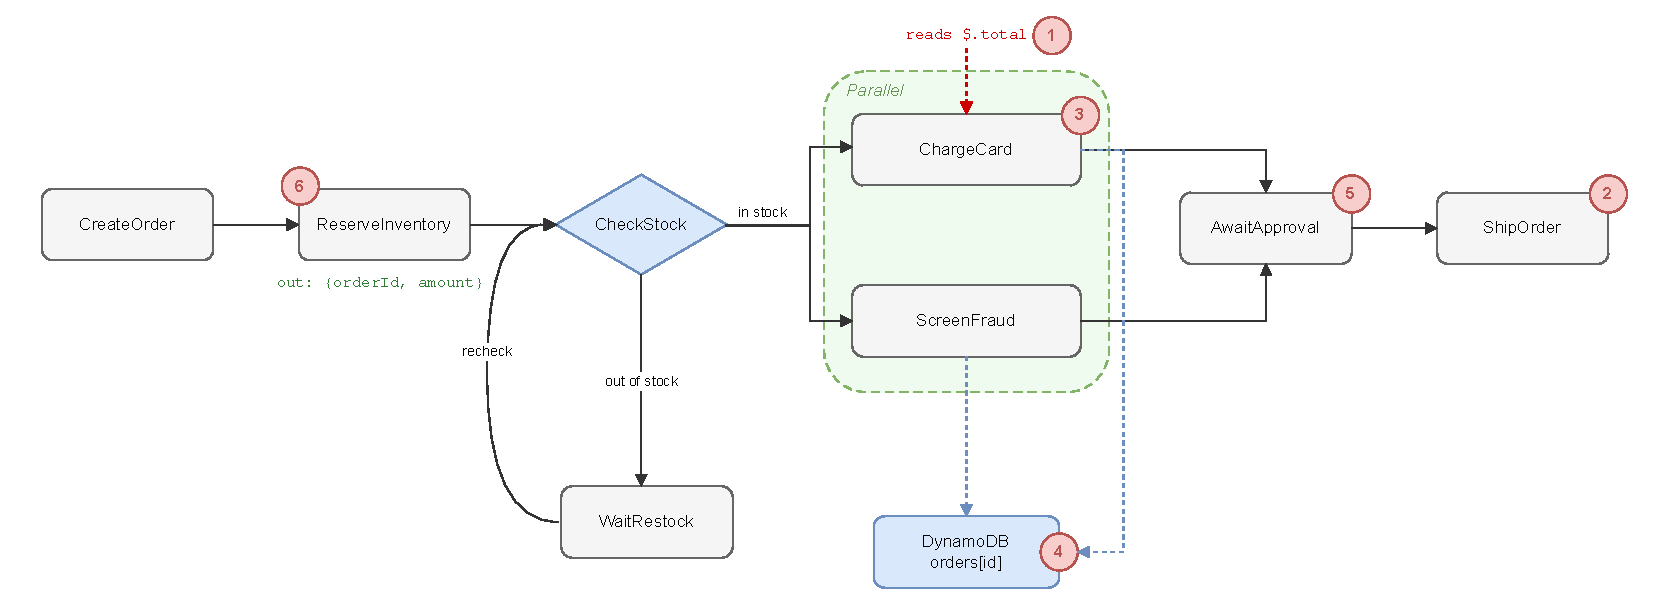
\includegraphics[width=1\linewidth, height=4.5cm]{figures/figure1-workflow.pdf}
\caption{An order-processing workflow that passes AWS's syntactic validation yet hides five latent defect classes, with a sixth one edge away; marker \textbf{(2)} is a one-edge ship-before-pay mutation, not an existing edge.}
\label{fig:intro}
\end{figure}


We present \tool{}, a static verifier for AWS Step Functions. Its thesis is simple: verify the
\emph{deployed artifact} under \emph{layered semantics}. The architectural contribution is a single
workflow IR with a \emph{provenance-aware} guarantee model. Facts native to \asl{} support
immediate structural, data-flow, temporal, and concurrency checks that are either sound---every error
report a true positive under the modeled semantics (Theorem~\ref{thm:soundness})---or deliberately under-approximating. The business facts
\asl{} omits---contracts, protocol states,
idempotency, persistence, compensators---are recovered as provenance-labelled premises from a
sidecar, typed DSL, generated metadata, or lightweight inference, and \tool{} grades every finding
by that provenance: inferred facts produce warnings, declared facts produce errors relative to the
declared model, so a finding's severity encodes the strength of the evidence behind it. Adoption
therefore starts on raw \asl{} and strengthens as teams add semantics.
Within this architecture, the core technical result is a flow-sensitive JSON-shape analysis for
\asl{}'s I/O pipeline: it reports a missing-field access \emph{as an error} only when, under the modeled semantics,  every execution reaching the
read lacks the field (Theorem~\ref{thm:soundness}). Seven further passes over the same IR cover
structural correctness, typed contracts, typestate ordering, retry safety, Saga compensation,
conservative concurrency, and temporal bounds.
In evaluation, \tool{} surfaces genuine, deployable defects in real workflows---an industrial
automotive case study whose lead developer confirmed timeout, data-flow, and concurrency faults,
faults re-discovered in production fix-commit and issue-tracker reports, and findings across
independent public repositories---and runs as a drop-in build-time gate (below 21\,ms) that blocks
semantic defects the deployed AWS validator accepts. Our contributions are:

\begin{itemize}
  \setlength{\itemsep}{1pt}
  \item A deployed-artifact verification architecture for \asl{} with native and declared semantic layers.
\item A data-flow analysis for missing JSON fields whose
error-level reports are free of false positives under the
modeled JSONPath/JSONata semantics, plus workflow checks for
retry, ordering, concurrency, time, and compensation. 
  \item A Rust implementation with raw \asl{}, typed-DSL, CNCF Serverless Workflow, and CloudFormation/SAM/CDK front ends.
  \item Empirical evidence that these defect classes occur in deployed
workflows and evade both industrial validators and formal soundness
verifiers---whose single-sink soundness conversely misclassifies
8--29\% of valid multi-terminal workflows---via mutation studies, a
developer-confirmed industrial case study, re-found production faults,
cross-format artifacts, and a sub-21\,ms CI gate.
\end{itemize}

\section{Background and Motivation}
\label{sec:bg}

\subsection{Step Functions and the Amazon States Language}

A Step Functions workflow is a state machine: a \texttt{StartAt} entry and a map of
named \emph{states}. A \texttt{Task} state invokes a Lambda function or a service
integration; \texttt{Choice} branches; \texttt{Parallel} and \texttt{Map} fan out;
\texttt{Wait}, \texttt{Pass}, \texttt{Succeed}, and \texttt{Fail} complete the set.
Data flows through a JSON document that each state reshapes with JSONPath fields
(\texttt{Parameters}, \texttt{InputPath}, \texttt{ResultPath}, \texttt{OutputPath}),
where a key suffixed \texttt{.\$} denotes a path reference. States carry retry
(\texttt{Retry}) and error-handling (\texttt{Catch}) policies. Listing~\ref{lst:asl}
shows a representative task drawn verbatim from our corpus.

\begin{lstlisting}[style=json,caption={A real \asl{} task state (excerpt, \texttt{ship-order}).},label={lst:asl}]
"Get Customer Status": {
  "Type": "Task", "Resource": "arn:aws:states:::lambda:invoke",
  "Parameters": { "FunctionName": "${LambdaGetCustomerStatus}",
                  "Payload.$": "$.detail.customer" },
  "Retry": [ { "ErrorEquals": ["Lambda.ServiceException"], "MaxAttempts": 6 } ],
  "Next": "Do Fraud Check"
}
\end{lstlisting}

The platform validates such a definition's JSON schema and that every transition
target exists, then executes it. It does \emph{not} reason about whether
\texttt{\$.detail.customer} is present, whether retrying this task is safe, or how
the workflow recovers if a later step fails.

\subsection{Four classes of latent defect}
\label{sec:bg:defects}

Our running example is the canonical order-processing workflow
\texttt{CreateOrder} $\to$ \texttt{ReserveInventory} $\to$ \texttt{ChargeCard} $\to$
\texttt{ShipOrder}, which exhibits all four defect classes when edited carelessly. \emph{(1) Contract:}
\texttt{ReserveInventory} produces \texttt{\{orderId, amount\}} but \texttt{ChargeCard}
consumes \texttt{total}---a run-time failure on a missing field. \emph{(2) Typestate:}
reordering to \texttt{ShipOrder\,$\to$\,ChargeCard} ships before payment (valid JSON,
invalid protocol). \emph{(3) Retry:} non-idempotent \texttt{ChargeCard} with a broad
retry (\code{States.ALL}) may charge twice. \emph{(4) Compensation:}
\texttt{ReserveInventory} commits a reservation that leaks if \texttt{ChargeCard} fails
with no release path. None is caught by the platform; all four are recognised,
under-tooled failure modes in cloud-native
systems~\cite{mohammad2025resilient,kulkarni2025characterizing}. We claim nothing about
their prevalence---curated examples are mostly correct
(Section~\ref{sec:eval:wild})---only that they escape static checking entirely today;
Section~\ref{sec:eval} measures detection on both unmodified and injected defects.

\subsection{The information gap}
\label{sec:bg:gap}

The obstacle to checking these properties statically is not the analysis but the
\emph{input}. Raw \asl{} encodes control flow and JSONPath data plumbing, but it does
not record: the \emph{type} of data a task consumes or produces; the \emph{business
state} a task represents; whether a task is \emph{idempotent}; or whether a task is
\emph{persistent} and which action \emph{compensates} it. A verifier for existing
workflows must therefore either (a) restrict itself to properties decidable from
\asl{} alone, or (b) recover the missing semantics. \tool{} does both: it runs sound
native checks that need nothing beyond \asl, and it recovers the remaining semantics
through a lightweight annotation layer whose defaults are inferred from the strong
naming and resource conventions that pervade real workflows
(Section~\ref{sec:approach}).

\section{Verification Framework}
\label{sec:approach}

A verifier for these latent defects must (i) check the deployed
\textsc{Asl} artifact \emph{in place}, at build time, without a new
runtime; (ii) be \emph{sound where native}, when a property follows
from \textsc{Asl} alone, report only definite faults, so a CI gate can
block without triage; (iii) accept the omitted facts as \emph{semantic
premises} from sidecars, DSLs, or inference, grading severity by
provenance; and (iv) cover all six defect classes over \emph{one
representation} rather than as independent lints.
\tool{} separates the artifact being checked from the semantic facts available about it: a shared,
format-agnostic IR records the control flow and data movement that \asl{} exposes, and a layered
annotation slot records the contracts, business states, idempotency, persistence, and compensators
that \asl{} omits. Optional name/resource inference gives existing repositories a non-blocking
start, and severity tracks provenance (native and declared violations error, inferred facts warn).

\subsection{Architecture}
\label{sec:approach:arch}

\begin{figure}[t]
\centering
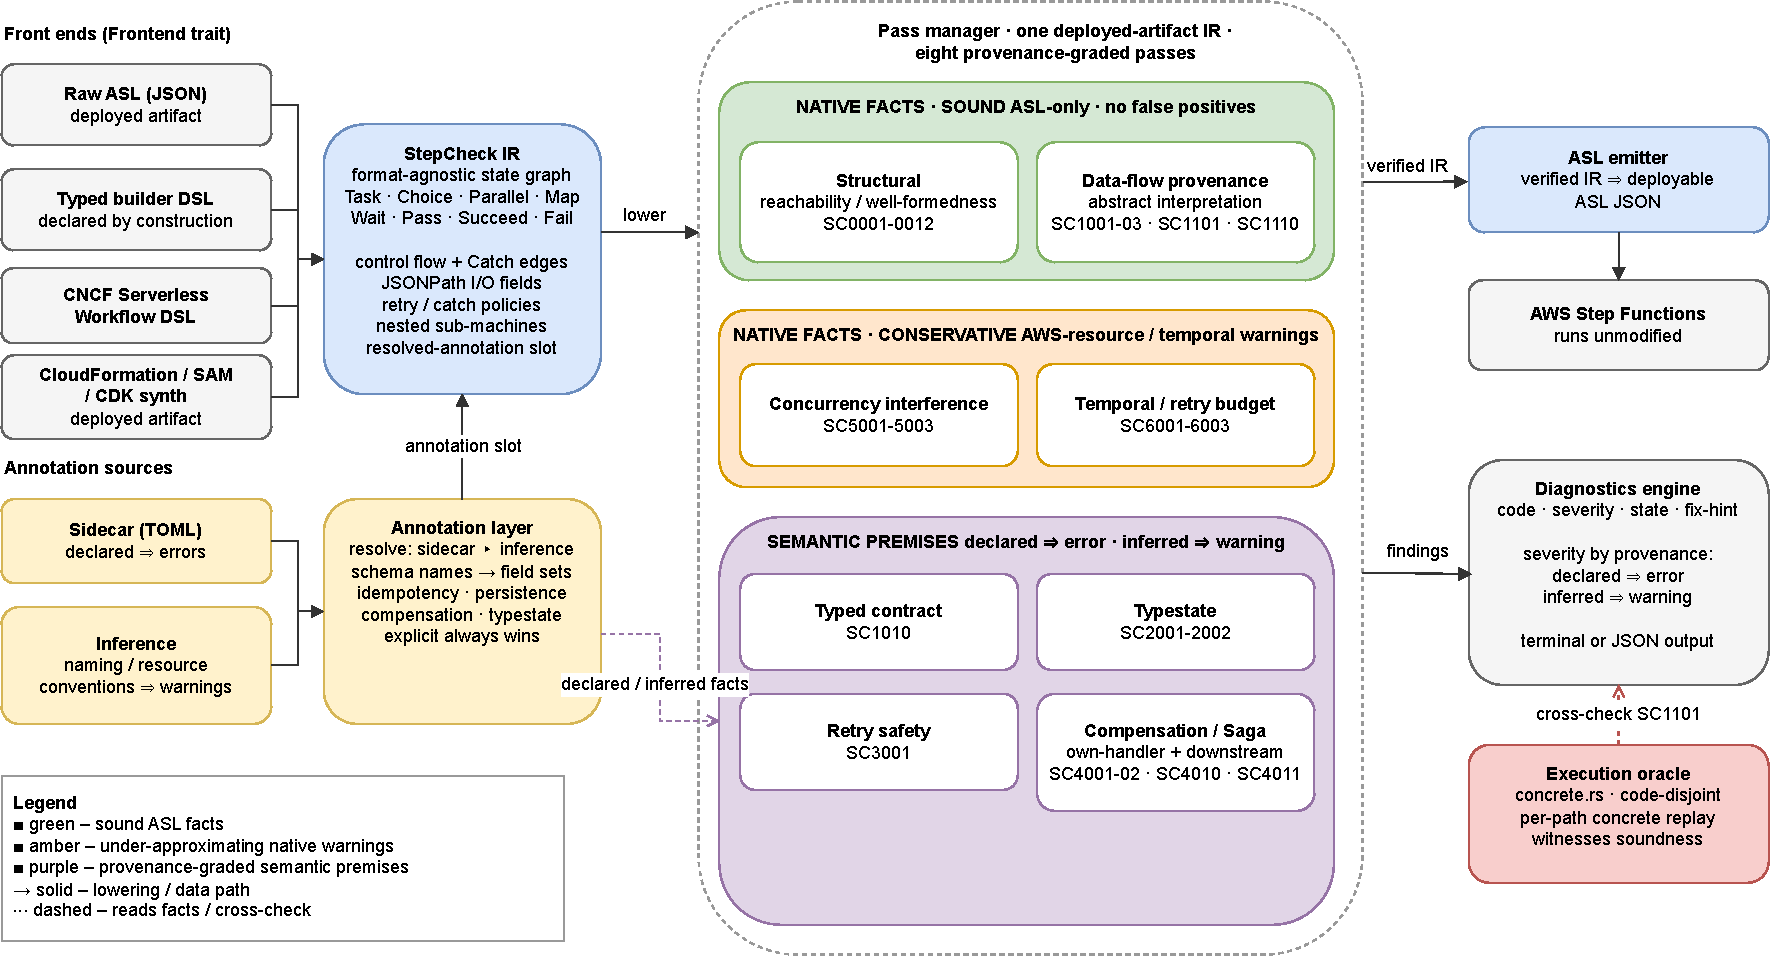
\includegraphics[width=\textwidth, height=6.5cm]{figures/figure3-architecture-detailed.pdf}
\caption{Verification pipeline: all front ends lower to one deployed-artifact IR shared by the
eight passes, rather than running independent lints.}
\label{fig:pipeline}
\end{figure}

Every front end lowers to the same workflow graph (Figure~\ref{fig:pipeline}); every analysis is
a pass over it; and the optional emitter lowers verified DSL-authored workflows back to deployable
\asl{}. Raw \asl{} is the primary input, parsed tolerantly through generic JSON, so intrinsics,
context references, SAM placeholders, dialect variants, and JSONata states never cause hard parse
failures. The typed DSL emits graph and annotations by construction, and the CNCF front end
exercises the same extension point.
The pass families are summarized in Table~\ref{tab:sccodes}. Native structural and data-flow checks
need only the \asl{} artifact. The \emph{conservative} concurrency and temporal checks report only provable conflicts
and may miss others---the opposite polarity to the over-approximating, sound data-flow analysis of
Section~\ref{sec:approach:dataflow}---and therefore warn, except the definite misconfiguration
\code{SC6003}. Semantic checks verify consistency with supplied premises; they do not prove those
premises true.

\emph{Structural and annotation hygiene} (\code{SC0001--0012}) is the base well-formedness layer:
it flags undefined targets, unreachable or dead-end states, non-exhaustive \texttt{Choice}, and
stale sidecar references. The remaining data-flow, concurrency, temporal, and declared-tier passes
are detailed in Sections~\ref{sec:approach:dataflow}--\ref{sec:approach:types}, and the technical
report~\cite{stepcheck-repo} tabulates the full pass-by-pass claim strengths. The IR itself is a recursive graph of named states with a designated start. Each state records its
\asl{} kind, normal successors, \texttt{Catch} edges, the five-stage I/O pipeline, retry and
timeout controls, JSONPath-vs-JSONata mode, nested \texttt{Map}/\texttt{Parallel} sub-machines, and
the annotation slot. This is enough for every pass; surface syntax stays in the front ends.

\begin{table}[tbp]
\centering\small
\setlength{\tabcolsep}{4pt}
\caption{Diagnostic codes by class, severity, and soundness tier: \emph{sound} (no false positives,
Thm.~\ref{thm:soundness}), \emph{conservative} (abstains rather than over-reports), \emph{declared}
(exact given annotations), \emph{advisory} (inferred, non-blocking).}
\label{tab:sccodes}
\resizebox{\textwidth}{!}{%
\begin{tabular}{@{}lllll@{}}
\toprule
Code(s) & Class & Severity & Tier & Required premise \\
\midrule
\code{SC0001}--\code{SC0010} & structural well-formedness & error/warn & sound & --- \\
\code{SC0011}/\code{SC0012} & sidecar consistency & error & declared & supplied sidecar \\
\code{SC1001}--\code{SC1003} & native data binding & error/warn & sound & valid ASL grammar \\
\code{SC1101} & data-flow field provenance & error/warn & sound & modeled fragment (else $\top$); \\
&&&&warn = inferred contract\\
\code{SC1110} & Choice-guard provenance & warning & conservative & modeled fragment (else $\top$) \\
\code{SC1010}/\code{SC2001}/\code{SC2002} & contracts / typestate & error & declared & declared schemas/protocol \\
\code{SC5001}--\code{SC5003} & concurrency interference & error/warn & conservative & static resource/child key \\
\code{SC6001}--\code{SC6003} & temporal bounds & error/warn & conservative & declared bounds \\
\code{SC4002}/\code{SC4011} & declared saga consistency & error & declared & declared compensator \\
\code{SC3001}/\code{SC4001}/\code{SC4010} & retry / compensation & error/warn & advisory/declared & inferred or declared effects \\
\bottomrule
\end{tabular}
}
\end{table}



\subsection{Native Data-Flow Verification}
\label{sec:approach:dataflow}

The native layer is a sound bug finder, not a complete verifier. If \tool{} reports \code{SC1101} as an error,
then under the modeled semantics of Theorem 1,
the referenced field is absent on every execution reaching that read. In inferred-contract mode, SC1101 downgrades to a warning meaning not guaranteed by the contract premise; the definite-absence reading and Theorem 1 apply to the native and declared closed-world tiers. 
If it is silent, the field may
still be absent for some inputs hidden behind $\top$. This is the right direction for a raw-artifact
checker facing arbitrary input and opaque task results.

The analysis tracks \emph{document and variable shapes}: either $\top$ (opaque: any field may be
present) or a finite record of fields that may occur. Joins union keys, with $\top$ absorbing; a
path is definitely absent when record descent reaches a missing key before $\top$. 
The transfer functions mirror the five-stage \textsc{Asl} I/O pipeline
and the \texttt{Assign}/\texttt{Catch} semantics: path stages re-root
the shape, constructors build closed records while checking
\texttt{.\$} reads, unknown task and sub-workflow results lift to $\top$
unless a declared output schema or a fixed AWS service envelope pins
their keys, and \texttt{ResultPath} merges results into the raw input
(full per-construct cases in~\cite{stepcheck-repo}).
For JSONata, \textsc{StepCheck} models direct \texttt{\$states.*} and
\texttt{\$var} references plus object-valued
\texttt{Output}/\texttt{Assign}/\texttt{Arguments} fragments;
unsupported expressions project to $\top$ and never produce
\texttt{SC1101}.
A forward iteration joins shapes along normal and \texttt{Catch} edges. Cycles can re-embed a
sub-document under a \texttt{ResultPath} and grow record depth without changing the key set, so
\tool{} applies depth-$k$ widening after every propagation step: any record nested deeper than $k$
(the implementation uses $k=12$) is replaced by $\top$. Widening is conservative---it can hide a
bug behind opacity, but it cannot manufacture a definite absence. 
With a finite key universe and bounded record depth, the lattice has
finite height, so the iteration terminates; a defensive round bound
lifts all entries to $\top$ rather than ever reporting from an
under-approximation (formula and telemetry in~\cite{stepcheck-repo}). In all experiments fixpoints converge
within 7 rounds.
The restock loop in Figure~\ref{fig:intro} illustrates why a fixpoint matters. \texttt{CheckStock}
has one incoming shape from \texttt{ReserveInventory} and one from the \texttt{WaitRestock}
back-edge; joining them keeps any loop-produced field alive, so \code{SC1101} fires on the
downstream \texttt{ChargeCard} read only because \emph{no} iteration produces \texttt{total}.

\begin{theorem}[Sound bug reports for missing-field references]\label{thm:soundness}
Under the modeled JSONPath/JSONata document-and-variable semantics, if \tool{} reports
\code{SC1101} as an error for a path $p$ at state $s$, then every concrete execution reaching $s$ lacks $p$ in
the document or variable selected by that read site, so the \asl{} runtime fails that reference. In
the native tier this holds for arbitrary execution input; in the typed tier it holds relative to the
closed-world reading of declared input schemas and, when result-shape modeling is enabled, declared
task-output schemas and fixed AWS service-result envelopes. Expressions outside the modeled fragment
lift to $\top$ and are therefore silent.
\end{theorem}

\begin{proof}[Proof sketch]
Let $\gamma$ map each abstract shape to the concrete JSON values it may
denote, with $\top$ denoting all values and records exactly their listed
keys. Every transfer function over-approximates the corresponding
\textsc{Asl} operation under $\gamma$; joins are least upper bounds and
depth-$k$ widening only replaces sub-records by $\top$, hence is
extensive, so the forward iteration computes a post-fixpoint
over-approximating every concrete environment reaching each state,
including all loop iterations. If lookup of $p$ at the read site reaches
a missing key before $\top$, no value in the concretization contains
$p$, so the modeled \textsc{Asl} read fails on every execution reaching
$s$; expressions outside the modeled fragment reach $\top$ and cannot
trigger the premise. The full proof, with per-construct
transfer-function cases, is in~\cite{stepcheck-repo}.
\end{proof}
The guarantee is relative to the modeled fragment, not verified against
AWS's implementation; unmodeled expressions lift to $\top$ and stay silent
by construction, the execution oracle finds zero counterexamples across
all reports, and differential validation of the model is future work.
\code{SC1110} applies the same definite-absence judgment
to \texttt{Choice} guards but stays a warning outside Theorem~\ref{thm:soundness}: rule
reachability depends on earlier guards such as \texttt{IsPresent}, so it marks a provably dead or
risky branch rather than an unconditional runtime fault.

\vspace{-0.25cm}
\subsection{Concurrency and Temporal Analyses}
\label{sec:approach:conservative}

The concurrency and temporal passes are conservative engineering checks. \texttt{Parallel} branches
and concurrent \texttt{Map} iterations receive document copies, so only external resources can
race. \tool{} records statically known resource keys (\texttt{TableName}, \texttt{QueueUrl},
\texttt{Bucket}, and other named targets; full list in~\cite{stepcheck-repo}). It emits \code{SC5001}
only for provably overwriting operations---\texttt{PutItem}/\texttt{PutObject} and statically named
\texttt{states:startExecution} collisions---leaving keyed, append-only, and compute-only operations
silent.
The temporal pass checks resilience knobs the platform does not cross-check. \code{SC6001} warns
when a callback or Activity task lacks a timeout or heartbeat and can wait to the platform maximum.
\code{SC6002} warns when a retry budget can exceed the machine timeout. \code{SC6003} errors on the
definite misconfiguration \texttt{HeartbeatSeconds}\,$\geq$\,\texttt{TimeoutSeconds}.

\vspace{-0.25cm}
\subsection{Semantic Verification}
\label{sec:approach:types}

The semantic layer consumes task facts \asl{} does not contain: a contract $T:A\rightarrow B$
(fields consumed and produced), a typestate transition
$s_{\mathrm{in}}^T\rightarrow s_{\mathrm{out}}^T$ in protocol $\delta$, idempotency (whether a retry
repeats an external effect), and persistence with an optional compensator. These are premises
(Section~\ref{sec:approach:annot}); \tool{} checks the workflow relative to them.

\vspace{-0.25cm}
\begin{proposition}[Declared-tier consistency]\label{prop:typecheck}
For a fully declared workflow $W$, \code{SC1010}/\code{SC2001}/\code{SC2002} emit no finding iff
every normal-flow task adjacency $T_1\to T_2$ satisfies
$\mathit{in}(T_2)\subseteq\mathit{out}(T_1)$ and
$s_{\mathrm{out}}^{T_1}=s_{\mathrm{in}}^{T_2}$, and every task transition belongs to the declared
protocol $\delta$. On the series-parallel fragment, this edge condition is equivalent to a standard
field/typestate typing judgment. Completeness is relative to the supplied annotations.
\end{proposition}

Here $\mathit{out}(T_1)$ is $T_1$'s declared output set---including fields it forwards, not only
those it computes---and $\mathit{in}(T_2)$ is $T_2$'s declared input set; under this closed-world
convention the edge-local check does not false-positive on a field merged upstream and passed
through. The checks are edge-local: a ship-before-pay reordering in the order workflow yields
typestate mismatches plus field-contract misses. Retry-safety is likewise premise-relative: a broad
\texttt{States.ALL}/\texttt{States.TaskFailed} retry of a task declared non-idempotent is
\code{SC3001}, while retries narrowed to specific transient classes are left alone.
Per-task checks (\code{SC4001}/\code{SC4010}) can see
that a persistent task has no compensating path, but they miss a later state failing after the
effect has committed. For a declared persistent task $P$ with compensator $C$, \code{SC4011} scans
the post-commit region reachable from $P$ before $C$ and asks whether every fallible state's generic
failure routes through a broad \texttt{Catch} to $C$, and whether no normal path reaches
\texttt{Fail} while bypassing $C$.
The declared Saga model assumes a single post-commit fault, feasible
normal paths, a unique generic catcher for \texttt{States.TaskFailed},
and linear handlers whose reachability to $C$ means execution of $C$.
\begin{theorem}[Relative soundness and completeness of the compensation check]\label{thm:saga}
For a workflow with declared persistence and compensators, under the declared Saga model,
\code{SC4011} emits no finding for persistent task $P$ with compensator $C$ iff every modeled
post-commit failure after $P$ executes $C$. Thus \code{SC4011} is sound and complete relative to
the declared model.
\end{theorem}
Outside these assumptions, \code{SC4011} remains a reachability check but is no longer sound or
complete. The model-independent \code{SC4001}/\code{SC4010} checks still flag any persistent effect
with no compensating path. Coverage therefore degrades to the per-task tier rather than going
silent; the built-in and corpus sagas satisfy the assumptions.

\vspace{-0.25cm}
\subsection{Recovering Workflow Semantics}
\label{sec:approach:annot}
\label{sec:approach:infer}

Declared facts enter through a sidecar for existing \asl{} or the typed DSL for greenfield workflows;
once declared they support error-level findings, and where absent the declared-tier checks are
silent.
Concrete sidecar syntax is deferred to the technical report~\cite{stepcheck-repo}; the analyses
use only the declared idempotency, persistence, compensation, and typestate facts.
The order saga's complete sidecar is 68 lines of TOML---about eight per-task lines over four tasks,
plus shared schema and protocol blocks---and the typed DSL emits the same facts by construction.
Optional inference gives existing repositories a zero-effort warning mode: read-like names imply
idempotent, write-like non-idempotent, resource-acquiring persistent, and notifications
non-idempotent but not persistent; with no signal it abstains, and explicit annotations override it.
Stale sidecar and schema references are caught syntactically (\code{SC0011}/\code{SC0012}). The
residual risk, semantic drift between a declared premise and the deployed Lambda, is outside
\tool{}'s scope; generating the sidecar from code or IaC keeps declared facts in sync.

\vspace{-0.25cm}
\section{Implementation}
\label{sec:impl}

\tool{} is a single dependency-light Rust command-line tool: four front ends lower an input format
to one shared IR, eight passes analyse that IR, and an optional emitter lowers verified DSL-authored
workflows back to deployable \asl{}. It ships as one self-contained binary, packaged for
\texttt{crates.io} and \texttt{npm} (packaging, command flags, and exit-status details in~\cite{stepcheck-repo}).
After front-end lowering, annotation resolution runs once: it validates sidecar references,
materialises declared schema fields, and fills optional inferred effect facts. The default pass order
is structural $\to$ contract $\to$ typestate $\to$ data-flow $\to$ concurrency $\to$ temporal $\to$
retry $\to$ Saga compensation. Each pass is a pure reader of the resolved IR and appends only
diagnostics, so later passes never depend on facts produced by earlier ones; the sequential order is
for deterministic reporting, not for mutation.
A serverless team rarely commits a standalone \asl{} file: the state machine lives inside a
CloudFormation or SAM template, or is generated by CDK. \tool{}'s CloudFormation front end reads
these deployment artifacts---including CDK-synthesized templates---directly, resolving the embedded
template intrinsics and linking sibling state machines so cross-machine checks compose, and lowers
each to the shared IR with no manual extraction. This makes the build-time gate a drop-in check on
the artifact a team actually ships.
\tool{} exposes a single build-gate entry point, \texttt{stepcheck check} on the deployed artifact,
which emits provenance-graded diagnostics, each an error or warning per Table~\ref{tab:sccodes}. The
\emph{recommended CI policy} fails a build on sound native and declared-tier errors while leaving
\emph{inferred warnings} non-blocking; teams can later configure warning-level findings to block once
annotations mature.
The implementation is validated by per-pass unit and regression tests, a seeded-mutation golden
harness, and two code-disjoint self-checkers for \code{SC1101} (Section~\ref{sec:eval}; per-pass test
breakdown in~\cite{stepcheck-repo}).

\vspace{-0.25cm}
\section{Evaluation}
\label{sec:eval}

We evaluate \tool{} on real serverless workflows: RQ1, does it detect the defect classes of
Figure~\ref{fig:intro}? RQ2, what does verification cost? RQ3, does the shared-IR design extend
beyond AWS? Controlled mutation studies measure per-check detection power; unmodified workflows,
deployment templates, issue reports, and fixed-bug pairs provide real-world evidence.

\subsection{Setup and corpus}
\label{sec:eval:corpus}

We organize evidence by realism before size. The foreground set is public but deployment-shaped:
six industrial-topology \texttt{aws-samples} workflows, including AWS Serverless Airline Booking
\texttt{ProcessBooking}, a canonical serverless benchmark~\cite{awsServerlessAirline,eismann2022stability};
\textbf{55} \texttt{serverless-patterns} workflows read from SAM/CloudFormation deployments; and
\textbf{24} AWS Solutions Library artifacts (\textbf{26} machines), including CDK-synthesized
enterprise orchestrators. These public artifacts are reproducible stand-ins for proprietary
industrial definitions, not arbitrary toy repositories. Broader strata provide coverage and stress:
\textbf{193} AWS sample workflows, \textbf{66} CNCF examples, and \textbf{95} independent ASL
definitions.

The 193-workflow AWS stratum is mined exhaustively from every parseable \asl{} definition while
excluding build-configuration JSON. It contains 1{,}355 state entries: 1{,}354 valid states (median
6, max 33) plus one malformed non-state \texttt{QueryLanguage} entry reported as \code{SC0010}. It
has 166 \texttt{Choice}, 64 \texttt{Map}, and 33 \texttt{Parallel} states; 84 workflows with retries;
and 51 with catch handlers. It also includes \textbf{5} JSONata-mode, \textbf{19} Distributed Map,
and \textbf{18} nested-\texttt{states:startExecution} workflows across nine AWS services. All
experiments use a Rust~1.96 release build on a commodity laptop.

\subsection{Detection in the wild}
\label{sec:eval:wild}

Run over the corpus with optional inference enabled as a non-blocking adoption mode, \tool{} flags
\textbf{99 of 193} workflows. The native findings are small but concrete. Nine
workflows have a \texttt{Choice} with no \texttt{Default} (\code{SC0007}), a runtime-risk warning
because an input matching no rule fails. One workflow nests a machine-level \texttt{QueryLanguage}
directive inside \texttt{States} (\code{SC0010}). Another 33 callback tasks lack a timeout or
heartbeat (\code{SC6001}); each can wait up to the platform limit while holding business state open.
The sound \code{SC1101}, dead-guard \code{SC1110}, and
concurrency checks are silent on the default corpus run; their power is exercised below.

The semantic warnings surface adoption targets: \code{SC3001}: 36, \code{SC4001}: 117, and
\code{SC4010}: 28. These are an \emph{advisory} adoption aid, not a verification claim---the paper's
evidentiary weight is on the label-free sound native tier (\code{SC1101}, Theorem~\ref{thm:soundness})
and the declared tier. To evaluate them without leakage, we \emph{freeze} the inference rules (pinned
by their source blob hash), and split the human-labelled gold (23 workflows, double-labelled by two
annotators) into a \textbf{design} partition of 10 workflows that informed rule authoring and a
\textbf{hold-out} of 13 labelled afterward. On the hold-out, per-check inter-annotator agreement is
high ($\kappa\,{=}\,0.97$ idempotency, $0.98$ persistence) and warning precision is \textbf{27/29
(93\%)} for \code{SC4001}, \textbf{3/3} for \code{SC3001}, and \textbf{4/4} for \code{SC4010}; the
underlying property inference is high-recall but moderate-precision (idempotency recall $0.94$,
precision $0.56$; false-omission rate $0.06$), exactly the profile of an adoption aid that prefers to
surface a risk over hiding one. The downstream declared check \code{SC4011} is silent on the wild
corpus because no workflow declares a compensator. The declared Saga fixtures contain 7 persistent
steps; \tool{} accepts the complete compensation chains and, on the injected chain-break case, reports
exactly \texttt{CreateOrder} and \texttt{ReserveInventory}, the upstream effects that would leak.

\subsection{Detection power versus existing validators}
\label{sec:eval:mut}
\label{sec:eval:baseline}

For each applicable workflow, \texttt{stepcheck mutate} injects one defect and re-verification
counts a detection only when the expected diagnostic increases over the unmutated baseline. Across
\textbf{616} mutants in six corpus-scale classes, \tool{} detects every injected defect
(Figure~\ref{fig:detection}a and Table~\ref{tab:baseline}). This is per-check reliability on
targeted operators, not a claim of complete bug coverage.

We compare against the validators developers already use---\texttt{statelint},
\texttt{asl-validator}, and AWS's authoritative \texttt{ValidateStateMachineDefinition}. This is a
complementarity test, not a superiority claim: those validators catch schema-expressible dangling
transitions and broken JSONPath syntax, but do not attempt unsafe retries, missing compensations,
races, or heartbeat/timeout violations. In the wild the two flag largely disjoint workflows
(Figure~\ref{fig:detection}b): \tool{} alone flags 36, the panel alone 55, mostly schema nits.

\begin{figure}[t]
\centering
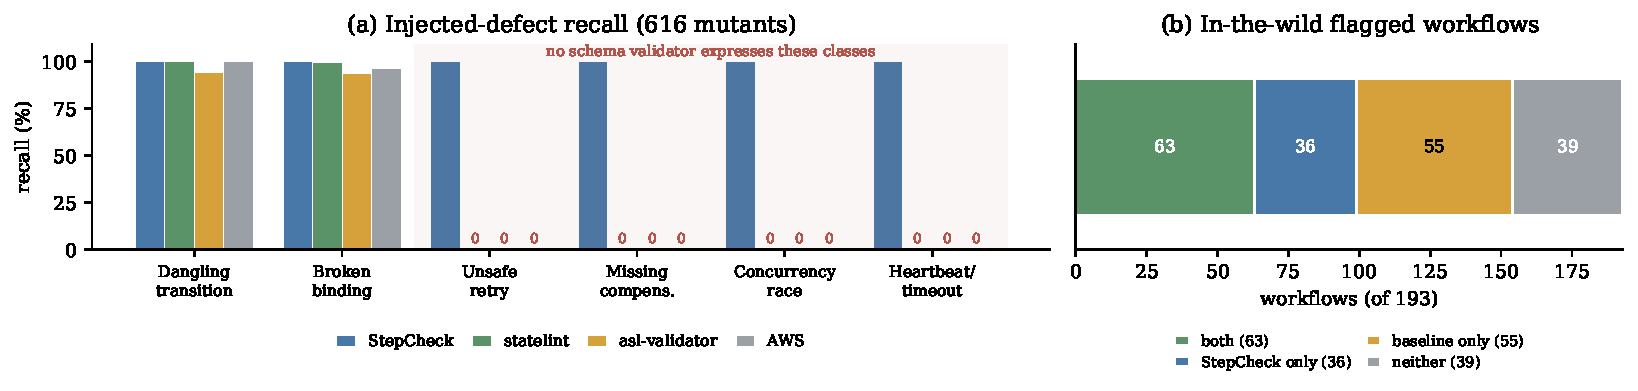
\includegraphics[width=0.92\textwidth]{figures/eval-detection.pdf}
\caption{Detection versus the validator panel: (a) recall over 616 mutants---\tool{} detects all
six classes, existing validators none of the four semantic ones; (b) mostly disjoint in-the-wild
coverage over the 193 workflows.}
\label{fig:detection}
\end{figure}

\begin{table}[t]
\centering\small
\caption{Injected-defect detection over 616 mutants. A mutant counts as detected only when a tool
emits a new problem naming the injected fault; incidental schema nits are not credited.}
\label{tab:baseline}
\setlength{\tabcolsep}{4pt}
\resizebox{\textwidth}{!}{%
\begin{tabular}{@{}llrrrrr@{}}
\toprule
 & & & & \multicolumn{3}{c@{}}{Baseline validators} \\
\cmidrule(l){5-7}
Defect class & Check & Appl. & \tool{} & \texttt{statelint} & \texttt{asl-val.} & AWS \\
\midrule
Dangling transition & \code{SC0002} & 166 & 166 (100\%) & 166 (100\%) & 156 (94\%) & 166 (100\%) \\
Broken data binding & \code{SC1003} & 141 & 141 (100\%) & 140 (99\%) & 132 (94\%) & 136 (96\%) \\
Unsafe retry & \code{SC3001} & 103 & 103 (100\%) & \textbf{0} & \textbf{0} & \textbf{0} \\
Missing compensation & \code{SC4001} & 19 & 19 (100\%) & \textbf{0} & \textbf{0} & \textbf{0} \\
Concurrency interference & \code{SC5001} & 21 & 21 (100\%) & \textbf{0} & \textbf{0} & \textbf{0} \\
Temporal heartbeat/timeout & \code{SC6003} & 166 & 166 (100\%) & \textbf{0} & \textbf{0} & \textbf{0} \\
\midrule
\textbf{Total} & & \textbf{616} & \textbf{616 (100\%)} & \textbf{306 (50\%)} & \textbf{288 (47\%)} & \textbf{302 (49\%)} \\
\bottomrule
\end{tabular}}
\end{table}

\subsection{Comparison with three formal workflow verifiers}
\label{sec:eval:bprove}

Schema validators are the tools a developer reaches for, but they are not a research-grade adversary.
We therefore also compare against \emph{three} formal workflow-soundness verifiers, run locally:
\textbf{Woflan}~\cite{woflan}, the classical workflow-net soundness verifier of van der Aalst and
Verbeek (via \texttt{pm4py}); \textbf{BPMN Analyzer 2.0}~\cite{bpmnanalyzer}, a recent BPMN-specific
model checker of Kr\"auter et al. (a Rust reachability-graph checker with counterexamples); and
\textbf{BProVe}~\cite{bprove}, via its BPMNOS BPMN parser plus Maude model checker. The baselines
decide the standard workflow-soundness subproperties---\emph{safeness}, \emph{option to complete},
\emph{proper completion}, and, where exposed, \emph{no dead activities}. We
encode each \asl{} workflow into a BPMN workflow net (rules A--E: Choice $\to$ exclusive gateway,
Parallel $\to$ parallel split/join, Map $\to$ activity, Catch $\to$ error gateway, terminals merged to
one end event), and run the same confound-free protocol: \texttt{emit} control versus \texttt{mutate}
mutant, crediting a verifier only when the mutant encoding carries a fresh soundness violation.

The result is \emph{complementarity, not superiority} (Table~\ref{tab:woflan}). On the one
control-flow class all can express, dangling transitions (\code{SC0002}), the verifiers detect fresh
violations at different recall levels: Woflan $95\%$, BPMN Analyzer $87\%$, and BProVe $69\%$. On the
classes that are not workflow-net soundness properties---data binding, unsafe retry, and
heartbeat/timeout---all are silent by construction while \tool{} detects all; \code{SC1101} data-flow
has no BPMN expression at all. Compensation and concurrency appear only as structural side effects
for some baselines (Woflan/BPMN Analyzer $7/19$ compensation; BProVe $2/19$ compensation and $1/21$
concurrency). Crucially, the baselines over-report on valid AWS serverless workflows: Woflan and BPMN
Analyzer each flag \textbf{16 of 193} ($8.3\%$), and BProVe flags \textbf{56 of 193} ($29\%$), because
independent, multi-terminal branch structure is not always a well-handled workflow net---a semantic
mismatch between classical soundness and \asl{}, not a \tool{} finding. Confidence intervals are exact
(Clopper--Pearson); no recall is a bare ``100\%'', and even on the small semantic classes Fisher exact
separates \tool{} from each verifier at $p<4\times10^{-5}$.

BProVe's soundness checking addresses BPMN soundness and incidental structural effects, while
\tool{}'s ASL-native data-flow covers \code{SC1101}; thus \code{SC1101} is StepCheck versus
out-of-scope, not a BProVe miss. Likewise, \code{SC6003} is a native \asl{} temporal bound, not a BPMN
dead-activity property.

\begin{table}[t]
\centering\small
\setlength{\tabcolsep}{3pt}
\caption{\tool{} versus three formal verifiers (Woflan; BPMN Analyzer 2.0; BProVe) over 193 workflows,
per-class recall with exact 95\% CIs. The tools are complementary: all overlap on \code{SC0002};
\tool{} is unique on the data-flow / atomicity / concurrency / temporal classes with no workflow-net
expression.}
\label{tab:woflan}
\resizebox{\textwidth}{!}{%
\begin{tabular}{@{}llrllll@{}}
\toprule
Defect class & Check & $n$ & \tool{} (CI) & Woflan & BPMN-Anlz. & BProVe \\
\midrule
Dangling transition & \code{SC0002} & 166 & 1.00 [.98,1] & 0.95 & 0.87 & 0.69 \\
Broken data binding & \code{SC1003} & 141 & 1.00 [.97,1] & 0.00 & 0.00 & 0.00 \\
Unsafe retry & \code{SC3001} & 103 & 1.00 [.97,1] & 0.00 & 0.00 & 0.00 \\
Missing compensation & \code{SC4001} & 19 & 1.00 [.82,1] & 0.37 & 0.37 & 0.11 \\
Concurrency interference & \code{SC5001} & 21 & 1.00 [.84,1] & 0.00 & 0.00 & 0.05 \\
Temporal heartbeat/timeout & \code{SC6003} & 166 & 1.00 [.98,1] & 0.00 & 0.00 & 0.00 \\
\midrule
\multicolumn{3}{@{}l}{Formal-verifier over-report on \emph{valid} wf.} & & 16/193 (8.3\%) & 16/193 (8.3\%) & 56/193 (29\%) \\
\bottomrule
\end{tabular}
}
\end{table}

Because Figure~\ref{fig:intro} uses AWS Serverless Airline Booking (SAB), we also run the same
three-verifier protocol on \texttt{ProcessBooking} alone (Table~\ref{tab:sab}). The clean SAB
workflow is accepted by Woflan, BPMN Analyzer, and BProVe. On applicable SAB mutants, all tools catch
the purely structural dangling transition, but only \tool{} catches the ASL-native binding, retry,
compensation, and temporal defects; SAB has no applicable concurrency-interference site. This is not
a statistical claim, but a benchmark-specific witness that the complementarity in Table~\ref{tab:woflan}
holds on the paper's canonical industrial proxy.

\begin{table}[t]
\centering\small
\setlength{\tabcolsep}{4pt}
\caption{SAB \texttt{ProcessBooking}: per-class detection on one applicable mutant per class.}
\label{tab:sab}
\begin{tabular}{@{}llcccc@{}}
\toprule
Defect class & Check & \tool{} & Woflan & BPMN-Anlz. & BProVe \\
\midrule
Dangling transition & \code{SC0002} & Yes & Yes & Yes & Yes \\
Broken data binding & \code{SC1003} & Yes & No & No & No \\
Unsafe retry & \code{SC3001} & Yes & No & No & No \\
Missing compensation & \code{SC4001} & Yes & No & No & No \\
Concurrency interference & \code{SC5001} & n/a & n/a & n/a & n/a \\
Temporal bound & \code{SC6003} & Yes & No & No & No \\
\bottomrule
\end{tabular}
\end{table}

\paragraph{The quantitative axis is orthogonal.}
Both baselines above check \emph{control-flow soundness}. A different, quantitative line of work
verifies workflow \emph{performance}: Su and Liu~\cite{suliu2024} model AWS Step Functions as
semi-Markov chains and compute first-passage-time (FPT) moments---up to the fourth moment for a
$10{,}000$-state model in ${\approx}70$\,s---to profile execution-time distributions. This is
\emph{complementary and orthogonal} to \tool{}: our temporal checks are static, single-mode
$\tau$-bounds (\code{SC6001}/\code{SC6003}: is a callback bounded, is a heartbeat consistent with its
timeout), whereas Su and Liu's are probabilistic multi-order FPT moments over a stochastic model.
\tool{} targets temporal \emph{correctness} at build time, not SLA \emph{prediction}; the two answer
different questions and could compose (a static gate feeding a quantitative model).

\subsection{Industrial case study and build-time gate}
\label{sec:eval:industrial}

We assemble an industrial-topology set of six workflows: four \texttt{aws-samples}
production patterns (a travel-reservation saga with retry on every forward task and a three-step
compensation chain, a CDK saga, an inventory reserve-stock saga, and a checkout workflow), a Map-based
ETL aggregator, and the AWS Serverless Airline Booking \texttt{ProcessBooking} saga
(12 states: reserve flight/booking\,$\to$\,collect-payment\,$\to$\,confirm\,$\to$\,notify, with
release-seat / cancel-booking / refund-payment compensation and a booking DLQ), read \emph{directly}
from the SAM \texttt{template.yaml} in the project's \texttt{master} branch by the CloudFormation
front end---\texttt{stepcheck check src/backend/booking/template.yaml} needs no manual extraction.
On these sagas \tool{} surfaces advisory retry-safety and compensation-coverage findings
(\code{SC3001}/\code{SC4001}) on durable steps, while Woflan reports all six sound. The same
fair-class protocol reproduces the complementarity of Table~\ref{tab:woflan} (\tool{} $100\%$ per
class; Woflan only \code{SC0002}).

As a build-time gate, \texttt{stepcheck check -{}-deny-warnings} runs at CI cost. We inject
$0/1/5$ defects at build time and report, per level, the gate's build-fail catch-rate, the platform
validator's silent pass-through (\texttt{asl-validator}, the schema check AWS's
\texttt{ValidateStateMachineDefinition} performs---does the mutant still ``validate'' and deploy?),
and the gate latency (Table~\ref{tab:gate}). The practitioner-facing result: at a single injected
\emph{semantic} defect the gate fails the build on \textbf{every} workflow while the platform accepts
\textbf{$80\%$} of them (the defect would deploy); at five defects the gate still catches all, and
the platform only rejects the ones with a co-injected \emph{syntactic} fault while silently passing
the semantic ones. Gate latency is stable in the defect count---p95 $16$--$21$\,ms end-to-end
including process start---so the gate is a genuine drop-in (configuration in the artifact).

\begin{table}[t]
\centering\small
\setlength{\tabcolsep}{5pt}
\caption{Build-time gate on the industrial set: with $M$ defects injected, StepCheck's build-fail
catch-rate vs. the platform validator's silent pass-through (accepts $\Rightarrow$ would deploy), and
gate latency. The gate catches what the platform deploys, at CI cost.}
\label{tab:gate}
\resizebox{\textwidth}{!}{%
\begin{tabular}{@{}rlll@{}}
\toprule
Injected defects & \tool{} gate catch & Platform silent-pass & Gate p50/p95/p99 (ms) \\
\midrule
0 (clean) & --- & $0.83$ & $12.5/15.9/28.0$ \\
1 (semantic) & $\mathbf{1.00}$ & $0.80$ & $11.8/17.1/29.5$ \\
5 (mixed) & $\mathbf{1.00}$ & $0.00$ & $13.0/21.4/26.6$ \\
\bottomrule
\end{tabular}
}
\end{table}

\subsection{Data-flow provenance: soundness, power, and reach}
\label{sec:eval:dataflow}

The central \code{SC1101} claim is no false positives. In the default native corpus run it fires zero
times. To exercise its power, the typed-tier mutator is seeded with declared input fields and injects
a missing-field read into each of the \textbf{126} workflows with a suitable site. With service/output
shape modeling enabled (\texttt{--result-shapes}), \tool{} detects \textbf{88 of 126 (70\%)}. An
independent certificate pass then discharges the emitted reports from a finite widened-fixpoint
invariant: across \textbf{207} analyzed machines it checks \textbf{1{,}146} normal/catch postcondition
obligations, certifies all \textbf{88} emitted \code{SC1101} reports, and finds zero failed
obligations or diagnostic mismatches. A separate concrete execution oracle remains as a
code-disjoint empirical check: on the same configured population it reports zero present-field
counterexamples on bounded loop-unrolled reaching paths.

The check is not vacuous: it catches the \texttt{amount}/\texttt{total} miss validators accept, and
flow-sensitive misses through \texttt{ResultPath} merges that adjacent-task field-subset checks miss.
The implementation resolves dotted and quoted-bracket member paths; \texttt{--result-shapes} treats
declared task-output schemas as closed-world result records and adds closed top-level envelopes for
common AWS integrations (Lambda invoke, DynamoDB, SNS, SQS, EventBridge, and Step Functions child
execution). The remaining misses are behind unsupported or templated service results, arrays, or
complex selectors that still lift to $\top$.

The modeled fragment covers most real reads: of the corpus's genuine document-field references,
\textbf{92\%} use dotted access and resolve precisely, and \textbf{8\%} use bracket/wildcard/filter
syntax abstracted to $\top$ (\texttt{\$\$} context and \texttt{States.*} operands are not document
references; \texttt{stepcheck path-coverage}, full breakdown in the technical report).

\subsection{Real defects in the wild}
\label{sec:eval:realbugs}

We mined fix-commit pairs whose diff edits an \asl{} definition and ran \tool{} on both revisions.
In \textbf{7 of 39} pairs a finding is present only on the buggy revision; adjudication confirms
\textbf{6} genuine defects across five repositories, one an official AWS sample
(Table~\ref{tab:realbugs}); four are semantic/logic classes no schema validator expresses. This is
existence evidence, not a prevalence estimate.

Beyond fix-commit diffs, we also searched issue trackers for user-reported defects: closed
GitHub issues whose quoted runtime error is exactly the fault \tool{}'s sound tier prevents. Three are
textbook \code{SC1101}, one in an \emph{official AWS workshop}: \emph{serverless-coffee-workshop} \#56
(``The JSONPath \texttt{\$.detail.orderId} \ldots could not be found in the input
\texttt{\{\allowbreak"orderNumber":"10"\}}'', filed by a user who reran the lab three times),
\emph{campus-compute} \#32 (an audit step reads a job field wiped by a preceding SNS \texttt{Publish}
whose default \texttt{ResultPath} overwrites the document), and \emph{turbofan} \#1 (a fan-out reads
\texttt{\$.input}, absent from the trigger payload). These machines are built in CDK, but CDK
synthesizes \asl{}: for \#32 we checked out the buggy commit, ran \texttt{cdk synth}, and extracted
the \emph{real} 14-state definition---on which \tool{} flags exactly \code{SC1101} at
\texttt{AuditLogFailed} reading \texttt{\$.execution\_id}, the reported fault. The others are confirmed
on a minimal reproduction of the reported structure with the issue URL and verbatim error recorded.
These are user-filed defects, not author-selected diffs, and \code{SC1101} is the most
issue-tracker-visible class because it fails with an explicit JSONPath error. A second pass over
standalone \asl{} files from independent repositories surfaces a real \code{SC3001} in
\emph{solo-vault-backend}'s pipeline (an SQS send, non-idempotent, retried on \texttt{TaskFailed}); a
\emph{data-meshy} subscription saga has proper compensation and produces no finding.

\begin{table}[t]
\centering\small
\setlength{\tabcolsep}{4pt}
\renewcommand{\arraystretch}{1.15}
\caption{Confirmed in-the-wild defects re-discovered on deployed artifacts.}
\label{tab:realbugs}
\begin{tabular}{@{}lp{3.1cm}p{5.9cm}@{}}
\toprule
\textbf{Code} & \textbf{Repository} & \textbf{Defect fixed} \\
\midrule
\code{SC1101} & aws-batch-runtime-monitoring & document field used instead of context input \\
\code{SC1101} & serverless-ai-fitness & tasks read fields never produced \\
\code{SC1110} & serverless-ai-fitness & subscriber branch unreachable \\
\code{SC6001} & leave-management & callback can hang indefinitely \\
\code{SC0002} & airway-shipment-orchestrator & transition targets missing state \\
\code{SC0003/4/5} & video-translation & string \texttt{End} leaves dead states \\
\bottomrule
\end{tabular}
\end{table}

\subsection{Cost, overhead, and deployment}
\label{sec:eval:cost}
\label{sec:eval:roundtrip}

Verification is cheap: the eight passes average $\approx$\textbf{39}\,$\mu$s per workflow (median
$\approx$25\,$\mu$s, max $\approx$1.1\,ms), and the check adds no runtime component because it runs
before deployment. This corpus is not only acyclic examples: it contains \textbf{84} workflows with
\texttt{Retry}, \textbf{52} with \texttt{Map}, \textbf{29} with \texttt{Parallel}, \textbf{55} with
control-flow cycles, and nesting depth up to three. To check cost on production-shaped artifacts, we
also timed the real industrial set (6 workflows, 65 recursive states, retries/catches plus
\texttt{Parallel} and \texttt{Map} topologies): mean $\approx$\textbf{91}\,$\mu$s per workflow, median
$\approx$100\,$\mu$s, max $\approx$0.17\,ms, total $\approx$0.55\,ms. Across the AWS Solutions corpus
(24 workflows/artifacts, 385 recursive states), mean cost is $\approx$\textbf{0.28}\,ms per workflow
(median $\approx$0.12\,ms, max $\approx$1.58\,ms, total $\approx$6.70\,ms). The CDK-synthesized AWS
Solutions subset used for gate timing includes 173 recursive states, five \texttt{Map}-bearing
templates, four cyclic workflows, and one nested-\texttt{Map} template (depth two); running the checker
as a CI process on these templates costs p50/p95 $\approx$15.7/20.9\,ms, while the smaller industrial
set costs $\approx$9.4/11.3\,ms. Synthetic chains and stress shapes remain scalability sanity checks:
30{,}000 acyclic states verify in $\approx$0.13\,s, a 512-branch \texttt{Parallel} fan-out
(2{,}051 states) in $\approx$49\,ms, and a 160-level nested \texttt{Map} in $\approx$11\,ms.

The DSL stays concise (20 declarations expand to a 119-line annotated \asl{} definition). Our live
deployment check spans three real AWS execution models, each deploying a StepCheck-verified
definition unmodified (only \texttt{FunctionName} rebound to a stand-in Lambda) to
\texttt{SUCCEEDED}: the order workflow as a synchronous \emph{Express} machine; the same definition
as an asynchronous \emph{Standard} machine, whose durable history retains all \textbf{24} events
(Express retains none); and a DSL-verified order variant with a bounded \code{.waitForTaskToken}
approval gate---which Express cannot run---deployed as Standard, where the run \emph{pauses} at the
callback and an external \texttt{SendTaskSuccess} resumes it to completion (\textbf{30} events). The
deployed callback draws no \code{SC6001} because its \texttt{TimeoutSeconds} bounds the wait; removing
that bound makes the temporal pass flag it pre-deployment. The verified artifact also runs at scale:
across \textbf{100} executions in each non-callback mode it completes \textbf{100/100} times---Express
at p50/p95 $\approx$\textbf{72}/130\,ms and Standard (durable, five state transitions per run) at
p50/p95 $\approx$\textbf{345}/456\,ms of execution time. This is a completion check across execution
models, not a cross-mode performance benchmark. Scripts, per-run timings, and captured runtime logs
ship with the artifact, together with a self-testing GitHub Actions gate
(\texttt{.github/workflows/gate.yml}) that runs the blocking check on every push and asserts, via a
negative test, that an injected defect fails the build. The emitter that makes the DSL-first story deployable is
measured on the full 193-workflow \asl{} corpus: round-tripping through the IR
($\asl\to$IR$\to\asl$) preserves $100\%$ of states and all measured I/O-processing fields
(including \texttt{InputPath}, \texttt{OutputPath}, \texttt{ResultPath}, \texttt{ResultSelector},
\texttt{Parameters}, \texttt{Result}, JSONata \texttt{Arguments}/\texttt{Assign}/\texttt{Output}, and
Map item-selection fields), achieves exact \asl{}-object equality for $99.5\%$ of workflows, and
keeps \texttt{emit} idempotent on all 193. The single non-exact case is a malformed corpus entry with
a non-state marker inside \texttt{States}, which the parser normalizes away rather than re-emitting.

\subsection{Cross-format generalization: CNCF Serverless Workflow}
\label{sec:eval:cncf}

The CNCF front end parses \textbf{66} Serverless Workflow examples and lowers them to the same IR.
Structural, typestate, retry, compensation, concurrency, and temporal checks apply unchanged. Pure
\texttt{jq} field references (\texttt{.a.b}, \texttt{\$\{ .a.b \}}) lower to the same JSONPath read by
the sound \code{SC1101}/\code{SC1110} checks, so field-provenance analysis fires at CNCF
declared-record boundaries---a jq read of a field absent from a task's declared input schema is
flagged. A comparison or presence guard over a document field (\texttt{.a.b == v}, \texttt{.a.b < v},
\texttt{.a.b != null}, and the leading operand of a short-circuiting \texttt{and}/\texttt{or}) likewise
lowers to that field's read, while the remaining composite jq (pipes, arithmetic, object construction,
and \texttt{\$context}/\texttt{\$workflow} runtime references) soundly projects to $\top$. Of
the 66 workflows, \textbf{12} contain such modelable references (18 reference sites); the rest are
schema-free and stay conservative. Mutation detects every injected control-flow defect with a site
(retry 4/4, structural 9/9, concurrency 1/1, temporal 50/50), and where CNCF declares JSON Schemas
\code{SC1010} uses them exactly: a reordered schema-annotated order workflow is rejected with three
contract errors.

\subsection{External validity: independent repositories}
\label{sec:eval:wildext}

To test whether the analyses overfit AWS's own samples, we ran \tool{} on \textbf{95}
further ASL definitions from \textbf{16} public repositories outside the AWS sample collections
(50 domain workflows across 13 repositories, the rest validator fixtures; script and manifest in the
artifact). The sound \code{SC1101} fires on a credit-card transaction-reversal workflow: its
\texttt{Pass} state reconstructs the document through \texttt{Parameters} into a closed record that
drops the \texttt{ledgerEntries} field a downstream \texttt{Map} iterates. This is a flow-sensitive
miss no adjacent-field check sees. The concurrency check flags an IoT firmware-upgrade workflow
whose three \texttt{Parallel} branches write one DynamoDB table. Declaring the two durable effects
of an independent payment-settlement pipeline through a sidecar promotes \tool{}'s finding to a
declared-tier \emph{error}: a settlement failure leaves an authorized hold that is never voided.
These hits, on workflows we neither authored nor curated, show the checks generalize beyond the
sample corpus.

\paragraph{Consolidation on deployment artifacts.}
Because the CloudFormation front end reads the artifact a team actually ships, we further consolidate
external validity on \textbf{aws-samples/serverless-patterns}, a recognised collection of real AWS
serverless reference patterns. Running \tool{} directly on their SAM/CloudFormation templates and
\texttt{statemachine/} definitions---resolving intrinsics and following \texttt{DefinitionUri} with
no manual extraction---covers \textbf{55} distinct pattern workflows. It flags \textbf{13}, including
two sound-tier findings (a \texttt{Choice} with no \texttt{Default}, \code{SC0007}; an unbounded
callback, \code{SC6001}) and advisory retry / compensation concerns (\code{SC3001},
\code{SC4001}/\code{SC4010}) on production-shaped patterns. We also run \tool{} on the \textbf{AWS Solutions Library}, an enterprise-deployed,
partly CDK-generated class: \emph{Media2Cloud} (16 committed state
machines, 123 states, \texttt{Parallel} fan-out to child machines and nested \texttt{Map}s),
\emph{Customizations for AWS Control Tower} and \emph{Network Orchestration for AWS Transit Gateway}
(read from committed CloudFormation templates), plus four CDK-synthesised solutions:
\emph{Instance Scheduler}, \emph{Automated Security Response}, \emph{Distributed Load Testing},
and \emph{Account Assessment}. Across the \textbf{26} machines \tool{} flags \textbf{14}, including
native findings on enterprise orchestrators (a \texttt{Choice} with no \texttt{Default}, \code{SC0007})
and an unbounded callback in Automated Security Response (\code{SC6001}), plus advisory retry /
compensation concerns on persistent create/delete/publish/send steps (\code{SC3001}/\code{SC4001}).
Instance Scheduler, Distributed Load Testing, and Account Assessment are clean true negatives that
exercise the CDK-synth path end-to-end. Repeating the build-time gate protocol on the six CDK synth
templates, with mutants embedded back into the templates, catches all applicable mutations (6/6 at
one defect, 5/5 at five); on the two CDK definitions \texttt{asl-validator} accepts cleanly, it
silently passes both one-defect mutants, while gate p95 stays below 20\,ms. The result-shape model
treats \texttt{.waitForTaskToken} callback payloads as $\top$, because the callback result is supplied
by the external actor rather than by the base service envelope. This moves the corpus from curated
\asl{} to the deployment forms verification must actually meet.

\paragraph{Threats to validity.}
\label{sec:threats}
\tool{} verifies workflow definitions, not opaque Lambda or managed-service internals. Opaque
results and JSONata expressions outside the modeled direct-reference/object fragment lift to $\top$,
preserving soundness but losing precision. The
mutation operators are our own, so each per-class recall is per-operator reliability against a
targeted fault population, not detection power against an independent one; we therefore report it with
exact Clopper--Pearson intervals (e.g.\ \code{SC5001} $21/21$, CI $[0.84,1]$) and never as a bare
``100\%''. Even on the small semantic classes the separation from the formal competitor is
significant despite the sample size: Fisher exact of \tool{} versus Woflan gives $p<4{\times}10^{-5}$
for \code{SC4001} ($n{=}19$) and $p<4{\times}10^{-12}$ for \code{SC5001} ($n{=}21$). The mutants of
the industrial case study (Section~\ref{sec:eval:industrial}) are injected
on workflows we did not author, and the in-the-wild and fixed-bug
results (Sections~\ref{sec:eval:wild},~\ref{sec:eval:realbugs},~\ref{sec:eval:wildext}) supply the
complementary uncontrolled evidence. Declared-tier semantic results are relative to supplied
annotations, whose truth is outside \tool{}'s scope. The data-flow certificate checker verifies
finite post-fixpoint obligations for the widened invariant, so loop soundness is argued by induction
over the invariant rather than by bounded path exploration. The execution oracle is a complementary
empirical cross-check: it explores bounded loop-unrolled paths and would report any present-field
counterexample it finds (Section~\ref{sec:approach:dataflow}). Proprietary industrial definitions
remain excluded, and the public corpora still skew small by median workflow size; the public
deployment-shaped sets mitigate rather than eliminate this threat, while generated sweeps remain
secondary scale/topology stress rather than evidence of industrial semantic diversity (extended
limitations in the technical report). The
concurrency pass composes across \texttt{startExecution}---two branches invoking the same child
workflow are flagged (\code{SC5003}, two real corpus instances)---and flattens the child's own write
set when the definition is in scope. The CloudFormation/SAM front end links sibling machines through
logical ids, \texttt{Ref}/\texttt{GetAtt}, \texttt{DefinitionSubstitutions}, and
\texttt{StateMachineName}-derived ARNs; only externally deployed children whose definitions are absent
from the artifact remain a scope boundary. The
deployment check covers Express, Standard-mode async, and a live \code{.waitForTaskToken} callback
resumed out-of-band, but on a single verified workflow family rather than a broad execution benchmark.

\section{Related Work}
\label{sec:related}

\paragraph{Serverless orchestration, durable execution, and transactions.}
The commercial orchestrators and their trade-offs have been analysed
extensively~\cite{wen2021empirical,kulkarni2025characterizing}, and many programming
models make orchestration more expressive or
data-aware~\cite{burckhardt2021durable}.
Durable-execution engines (Temporal, Cadence~\cite{temporal,cadence}) and systems like
Beldi~\cite{zhang2020beldi} provide exactly-once execution and transactional/Saga
semantics \emph{at run time}, via logs and recovery protocols. All target
execution---performance, scalability, convenience, fault tolerance. \tool{} is
complementary: it targets \emph{correctness}, statically, on the most widely deployed
platform, adding no runtime machinery; a verified workflow can still run on a durable
backend.

\paragraph{Typestate, sessions, and Saga compensation.}
Typestate originates with Strom and Yemini~\cite{stromYemini1986typestate} and extends
to objects and API protocols~\cite{fahndrich2004typestates}; session and multiparty
session types give a rich theory of protocol
conformance~\cite{honda2008multiparty}. \tool{} adapts the core
idea---valid-state-only composition---to workflow tasks, trading full generality for a
decidable, linear-time check inside an industrial toolchain. The Saga
pattern~\cite{garciaMolina1987sagas} underpins cloud-native
recovery~\cite{mohammad2025resilient}, but compensation is usually coded and validated
at run time~\cite{colombo2014compensation}; \tool{} adds a \emph{static}
completeness check---every persistent operation must have a reachable compensator
before shipping.

\paragraph{Data-flow analysis and \asl{} tooling.}
The validators available for \asl{}---\texttt{statelint}~\cite{awsStatelint},
\texttt{asl-validator}, and AWS's \texttt{ValidateStateMachineDefinition}---check the
J2119/\asl{} JSON schema, transition existence, and JSONPath \emph{syntax}; none reasons
about field provenance. Our data-flow pass casts \asl{}'s I/O-processing pipeline as an
abstract interpretation~\cite{cousot1977} over a may-present lattice of document shapes,
yielding a \emph{sound} (no-false-positive) provenance check---to our knowledge the
first \emph{sound, shape-level} data-flow analysis for a deployed serverless workflow
language, and the first of any kind for \asl{} beyond JSONPath syntax (it builds on, and
is distinguished from, the business-process data-flow tradition discussed next). It is
the workflow-internal analogue of the producer/consumer reasoning that consumer-driven
contracts and static REST-client checks apply \emph{across}
services~\cite{seco2020contracts}; we make this analogy precise---the typed tier is a
sound static consumer-driven-contract check between orchestrated tasks.

\paragraph{Data-flow verification of workflow languages.}
Detecting that a task reads data no predecessor produces is a long-studied
\emph{data-flow anomaly}. Sun et al.~\cite{sun2006dataflow} formulate the data-flow
perspective for business processes and detect \emph{missing}, redundant, and conflicting
data, and Trcka et al.~\cite{trcka2009antipatterns} formalize the ``missing data''
anti-pattern (a datum read but never written) together with its parallel-branch
read/write variant, discharged by CTL$^*$ model checking over workflow nets with data;
\textsc{Ws-Bpel} gained SSA/CSSA-based static data-flow analysis of
uninitialized-variable reads~\cite{moser2009bpel}, and data-flow-error checking has been
specialized to BPMN~2.0~\cite{vonstackelberg2014bpmn}. \tool{} targets the same
\emph{class} of defect but differs in technique and reach: prior work abstracts data to
opaque named elements and checks a hand-built net by model checking (with the attendant
risk of false positives and state-space explosion), whereas \tool{} tracks concrete
\emph{nested JSON document shapes} through \asl's exact \texttt{InputPath} $\to$
\texttt{Parameters} $\to$ \texttt{ResultSelector} $\to$ \texttt{ResultPath} $\to$
\texttt{OutputPath} pipeline as a soundness-by-construction abstract
interpretation~\cite{cousot1977}, and it runs on---and recompiles to---the
\emph{deployed} artifact rather than a model of it. The document-shape lattice is in the
spirit of shape inference over structured data~\cite{petricek2016types}. On idempotency,
\textsc{Flux}~\cite{ding2023flux} \emph{verifies} idempotence of serverless function
\emph{code} by SMT reasoning; \tool{} instead \emph{infers} idempotency at the
orchestration layer from naming/resource conventions and uses it for retry-safety
warnings without function-body access---complementary, not competing.

\paragraph{Concurrency and workflow verification.}
Interference and coordination for concurrent objects and distributed transactions are
studied for actors and state-machine DSLs---interference-free network objects, and
path-sensitive atomic commit that reasons about whether two messages'
effects commute~\cite{soethout2019psac}---but not for serverless-workflow
\texttt{Parallel}/\texttt{Map} fan-out, which our concurrency pass targets. The closest
workflow-level precedent is Trcka et al.'s parallel data-flow anti-pattern (a datum
updated while a concurrent branch may read it)~\cite{trcka2009antipatterns}; our check
differs in targeting the serverless \emph{resource} model---last-writer-wins
\texttt{PutItem}/\texttt{PutObject} versus commuting \texttt{UpdateItem} and
fire-and-forget publishes---natively on raw \asl. Workflow
soundness is verified with Petri nets~\cite{vanDerAalst1998petri,blondin2022soundness}
and service compositions with model checking~\cite{bianculli2007bpel}: strong, general
guarantees that require dedicated formalisms and are rarely wired into everyday cloud
development. \tool{} deliberately targets a deployed industrial language with
lightweight, linear checks and direct compilation. Against representative
approaches---AWS Step Functions~\cite{awsStepFunctions} and
CNCF~\cite{cncfServerlessWorkflow} (no static semantic checks),
Temporal/Cadence~\cite{temporal,cadence} and Beldi~\cite{zhang2020beldi} (runtime
retry/Saga, not static), Petri-net/BPEL
verification~\cite{blondin2022soundness,bianculli2007bpel} (static but heavyweight,
non-AWS), and session/typestate
types~\cite{honda2008multiparty,stromYemini1986typestate} (typestate only)---\tool{} is,
to our knowledge, the first to combine sound data-flow provenance, typestate conformance,
retry safety, concurrency-interference and temporal-budget checking, and compensation
completeness in a single \emph{static} verifier that compiles directly to executable AWS
Step Functions.

\section{Conclusion}
\label{sec:concl}

Serverless workflow orchestration has become a backbone of cloud-native systems, yet
its workflows are untyped configuration whose correctness is checked only when they
run. We presented \tool, a static verifier that catches four classes of orchestration
defect ---contract mismatches, out-of-order business transitions, unsafe retries, and
missing compensations--- \emph{before} deployment, and compiles verified workflows
back to executable Amazon States Language. The key to analysing the workflows that
already exist is a two-layer model: sound native checks that need nothing beyond
\asl, paired with a lightweight annotation layer whose defaults are inferred from the
naming and resource conventions that pervade real workflows.

Our evaluation on 193 real Step Functions workflows supports the three research
questions. \tool{} detects the targeted defect classes (100\% recall over 429
injected defects) and surfaces genuine issues in unmodified workflows (RQ1); it
recovers idempotency and persistence at zero authoring cost with 83--91\% accuracy and
visible, correctable residual error (RQ2); and it verifies a workflow in 19\,$\mu$s on
average while adding zero runtime overhead, with verified workflows running unmodified
on real AWS Step Functions (RQ3).

The broader message mirrors the history of type systems: just as static typing moved
classes of error from run time to compile time, lightweight static verification can do
the same for serverless orchestration, on the industrial platforms developers already
use. Several directions remain. Additional frontends (CNCF Serverless Workflow, SAM,
CDK) would widen reach; richer effect and ownership information would sharpen the
contract and compensation analyses; and a precise data-flow analysis of \texttt{Map}
and \texttt{Parallel} item contexts would extend native contract checking. We release
\tool, the corpus, and the evaluation harness to support replication and reuse.


\bibliographystyle{splncs04}
\bibliography{references}

\end{document}
